\documentclass[a4paper,11pt,french]{article}
\usepackage[utf8]{inputenc}

\usepackage[T1]{fontenc}
\usepackage[francais]{babel} 
\usepackage[top=2cm, bottom=2cm, left=2cm, right=2cm, includeheadfoot]{geometry} %pour les marges
\usepackage{lmodern}
\usepackage{pict2e}
\usepackage{tikz}	
\usepackage{tikz-uml}
\usepackage{fancyhdr} % Required for custom headers
\usepackage{lastpage} % Required to determine the last page for the footer
\usepackage{extramarks} % Required for headers and footers
\usepackage{graphicx} % Required to insert images
\usepackage{tabularx, longtable}
\usepackage{color, colortbl}
\usepackage{lscape}
%\usepackage[hidelinks]{hyperref}
\usepackage{longtable}
\usepackage{multirow}
\usepackage{rotating}
\usepackage{gensymb}
\usepgflibrary{arrows} % for pgf-umlsd

\usetikzlibrary{trees,shapes.geometric,arrows,decorations.pathmorphing,backgrounds,fit,positioning,shapes.symbols,chains	}

\linespread{1.1} % Line spacing

% Set up the header and footer
\pagestyle{fancy}
\lhead{\textbf{\hmwkClass -- \hmwkSubject \\ \hmwkTitle \\ \hmwkDocName}} % Top left header
\rhead{
\includegraphics[width=10em]{logo_univ.png}}
\lfoot{\lastxmark} % Bottom left footer
\cfoot{} % Bottom center footer
\rfoot{Page\ \thepage\ / \pageref{LastPage}} % Bottom right footer
\renewcommand\headrulewidth{0.4pt} % Size of the header rule
\renewcommand\footrulewidth{0.4pt} % Size of the footer rule

\setlength{\headheight}{40pt}

\newcommand{\hmwkTitle}{Transchiffrement} % Assignment title
\newcommand{\hmwkClass}{Master 2 SSI } % Course/class
\newcommand{\hmwkAuthorName}{Yves Nouafo} % Your name
\newcommand{\hmwkSubject}{Conduite de projet} % Subject
\newcommand{\hmwkDocName}{Collisions MD5} % Document name

\newcommand{\version}{1.0} % Document version
\newcommand{\docDate}{2 Janvier 2014} % Document date
\newcommand{\checked}{} % Checker name
\newcommand{\approved}{Magali Bardet} % Approver name

\makeatletter
\newcommand{\resettranslate}{\let\translate\@firstofone}
\makeatother

\definecolor{gris}{rgb}{0.95, 0.95, 0.95}

\title{
\vspace{2in}
\textmd{\textbf{\hmwkClass :\ \hmwkTitle}}\\
\normalsize\vspace{0.1in}\small{Due\ on\ \hmwkDueDate}\\
\vspace{0.1in}\large{\textit{\hmwkClassInstructor\ \hmwkClassTime}}
\vspace{3in}
}

\author{\hmwkAuthorName}
\date{} % Insert date here if you want it to appear below your name


\usepackage{amsmath}
\begin{document}
\newcount\startdate
\newcount\daynum
%\pgfcalendardatetojulian{2013-01-021}{\startdate}
\pagestyle{fancy}

\vspace*{5cm}
\begin{center}\textbf{\Huge{\hmwkDocName}}\end{center}
\vspace*{4.5cm}
	

\fcolorbox{black}{gris}{
\begin{minipage}{15cm}
\begin{tabularx}{10cm}{lXl}
	\bfseries{Version} & & \version\\
	& & \\
	\bfseries{Date} & & \docDate\\
	& & \\
	\bfseries{Rédigé par} & & \hmwkAuthorName \\
	& & \\
	\bfseries{Relu par} & & \checked \\
	& & \\
	\bfseries{Approuvé par} & & \approved \\
	& & \\
\end{tabularx}
\end{minipage}
}

\newpage

%Tableau de mises à jour
\vspace*{1cm}
\begin{center}
\textbf{\huge{MISES À JOUR}}\\
\vspace*{3cm}
	\begin{tabularx}{16cm}{|c|c|X|}
	\hline
	\bfseries{Version} & \bfseries{Date} & \bfseries{Modifications réalisées}\\
	\hline
	1.0 & 02/01/2014 & Création\\
	\hline
	& & \\
	\hline
	\end{tabularx}
\end{center}

%La table des matières
\clearpage
\tableofcontents
\clearpage

\section{Introduction}
Ces dernières années, le progrès en terme de sécurité informatique a été fulgurante. Plusieurs méthodes de cryptographie ont été développée. Ces méthodes moderne repose sur les fonctions de hachages cryptographiques. Ce sont des fonctions qui associent à un message de longueur arbitraire une chaine d'octets de longueur fixe appelé {\it{hashé}}.\\

Les fonctions de hachage doivent satisfaire les principes suivant:
\begin{itemize}
  \item résistante au calcul de collision
  \item résistante au calcul de seconde pre-image
  \item résistante au calcul de pré-image
\end{itemize}
\vspace{.5cm}

Une des fonctions de hachage les plus utilisés est MD5, inventé par Rivest en 1992. MD5 comme toute fonction de hachage prend en entrée un message de longueur variable et retourne une chaine de 128 bits.\\

Le but de cette étude est de décrire le fonctionnement interne de la fonction de hachage MD5 et d'en réaliser un état de l'art sur sa résistance aux collisions. Plus précisément, comment générer des entrées différentes pour la fonction MD5 de telle sorte que ces deux entrées aient le même hashé MD5.\\
Dans une étude plus approfondie, nous verrons comment il est possible d'appliquer l'étude à un cas pratique: La collision sur des fichiers.\\


\section{Préliminaire}
Comme la plupart des fonctions de hachage, MD5 est dotée d'une fonctionde compression qui s'appuie sur le fonctionnement de Merkle-Damgard, dont le principe est le suivant:\\
\begin{itemize}
\item La fonction de compression prend en entrée un bloc B de taille 512 bits et une IHV (valeur de hachage intermmédiaire) de 128 bits
\item Chaque message passé en paramètre doit subir un padding si sa taille n'est pas multiple de 512.
\item Le message (complété ou non) est ensuite découpé en N blocks de 512 bits.
\item La fonction de hachage commence avec un IHV initial appelé {\it{IV}} (initial value).
\item pour chaque bloc de message $M_{i}$ la fonction de compression de est appelé avec la valeur courante $IHV_{i}$ et calcul une nouvelle valeur $IHV_{i+1}$. Lorsque tout les blocs sont traité le {\it{hashé}} final $IHV_{N}$ est construit.
\end{itemize}
\vspace{.5cm}

Le schéma de fonctionnement est le suivant:

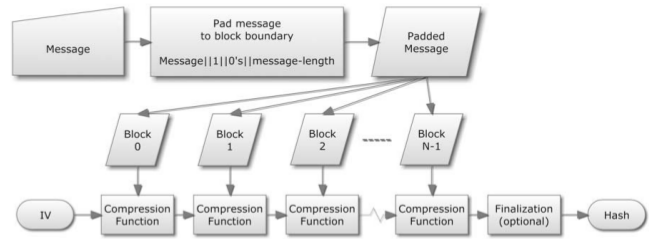
\includegraphics[scale=.61]{md.png}

\section{Fonctionnement de MD5}
Comme nous l'avons vu dans la section précédente, on sait que MD5 suit le schéma de construction de Merkle-Damgard et fonctionne de la manière suivante:\\
\begin{enumerate}
\item {\it{le padding}}. Si la longueur du message n'est pas un multiple de 512, on ajoute un pad, dont le premier bit est à 1 suivi de 0 de telle sorte que la longueur résultante soit égale à 448 mod 512. Les bits restants sont utilisés pour ajouter la longueur du message initial ;
\item {\it{le partitionnement}}. MD5 découpe le message original résultant d'un padding ou non en N blocs $M_{i}$, ...,$M_{N}$ de 512 bits ;
\item {\it{le processus}}. MD5 calcule des valeurs intermémdiaire de hash, {\it{IHV}}. Chaque IHV est diviser en 4 mots de 32 bits (a, b, c, d). ($a_{0}$, $b_{0}$, $c_{0}$, $d_{0}$) = ($67452301_{16}$, $EFCDAB89_{16}$, $98BADCFE_{16}$, $10325476_{16}$) sont des valeurs publiques initiales fixées,  chaque IHV calculée en utilisant la fonction de compression MD5Compress comme suit:\\ $IHV_{i}$ = MD5($IHV_{i-1}$, $M_{i}$) ;
\item {\it{le résultat}}. La valeur du hash résultant est la dernière valeur IHV calculée. Cet IHV est la concaténation en hexadécimal des dernières valeurs (a, b, c, d) calculés.
\end{enumerate}

\section{La fonction de compression MD5}
La fonctionde compression de MD5 prend en paramère une IHV de 128 bits et un bloc de message de 512 bits. Elle s'effectue en 64 étapes découpés en 16 tours. Chaque étape est munies d'opérations telle que l'addition,\\
la rotation gauche RC telle que:\\
\vspace{.5cm}
($RC_{t}$, $RC_{t+1}$, $RC_{t+2}$, $RC_{t+3}$) =
$\left\{
\begin{array}{l}
  (7, 12, 17, 22)   \hspace{.8cm}pour \hspace{.2cm} t = 0, 4, 8, 12 \\
  (5, 9, 14, 20)  \hspace{1cm}pour \hspace{.2cm} t = 16, 20, 24, 28 \\
  (4, 11, 16, 23)  \hspace{.8cm}pour \hspace{.2cm} t = 32, 36, 40, 44 \\
  (6, 10, 15, 21)  \hspace{.8cm}pour \hspace{.2cm} t = 48, 52, 56, 60 \\
\end{array}
\right.$
\vspace{.5cm}

une fonction non-linéaire $f_{t}$ telle que:\\
\vspace{.5cm}

$f_{t}$(x, y, z) =
$\left\{
\begin{array}{l}
  F(x, y, z) = (x  \bigwedge y) \bigoplus (\bar x \bigwedge z) \\
  G(x, y, z) = (z  \bigwedge x) \bigoplus (\bar z \bigwedge y) \\
  H(x, y, z) = x \bigoplus y \bigoplus z \\
  I(x, y, z) = y \bigoplus (x \bigvee \bar z) \\
\end{array}
\right.$
\vspace{.5cm}

Le bloc de message B est coupé en 16 mots consécutif $M_{0}$, ..., $M_{15}$ et étendu à 64 mot $W_{t}$ pour 0 <= t <= 64 de 32 bits chacun telle que:
\vspace{.5cm}

$W_{t}$ =
$\left\{
\begin{array}{l}
  réecritre les mt\\
\end{array}
\right.$
\vspace{.5cm}

En suivant la description de la fonction de hachage de MD5, pour chaque étape {\it{t}}, l'algorithme de fonction de compression sauvegarde un registre avec 4 états de mots $Q_{t}$, $Q_{t-1}$, $Q_{t-2}$, $Q_{t-3}$ et calcul un nouveau mot $Q_{t+1}$. On a alors l'initialisation suivante:\\
($Q_{t}$, $Q_{t-1}$, $Q_{t-2}$, $Q_{t-3}$) = (b, c, d, a)\\
for{\it{t}} = 0, 1, ..., 63, $Q_{t}$ est calculé comme suit:
\vspace{.5cm}

$\left\{
\begin{array}{l}
  F(t) = f(t)(Q(t), Q(t-1), Q(t-2) \\
  T(t) = F(t) + Q(t-3) + AC(t) + W(t) \\
  R(t) = RL(T(t), RC(t)) \\
  Q(t+1) = Q(t) + R(t) \\
\end{array}
\right.$
\vspace{.5cm}

\section{Présentation d'une collision à prefixe choisi}
Cette partie s'inspire des travaux réalisés par Marc Stevens célèbre cryptologue. Marc Stevens reprend les travaux réalisés par Wang et Yu et améliore ainsi leur algorithme en y introduisant d'autre notions et montre comment à partir de deux messages arbitraires, il est possible de générer des collisions sous MD5. Les algorithmes implémentés sont ceux décrit par Stevens. Mais avant tout une brève explication de la méthodologie de Stevens.

\subsection{Vue sur les préfixes choisis}
Les deux messages initiaux peuvent avoir des longueur différentes. Dans ce cas, il faut appliquer un padding au plus court des deux, pour qu'elles aient des longueurs égales. En agissant de la sorte, lorsque les message seront passé à la fonction de compression de MD5, on s'assure que qu'ils auront le même padding. \\
///////////////////////////////////////////////////////////\\
////////////// COMPLETER ///////////////////\\
///////////////////////////////////////////////////////////\\

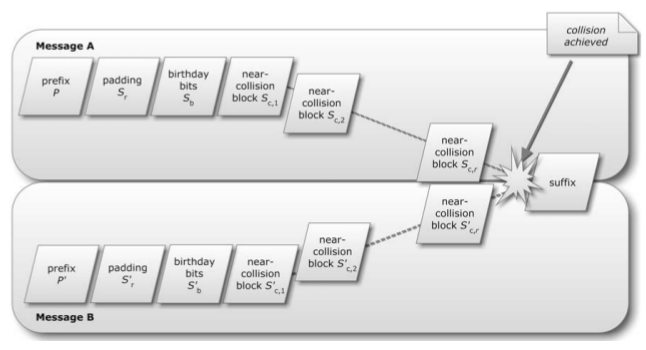
\includegraphics[scale=.61]{col.png}


\subsection{Construction des préfixes choisis de collisions}
Un préfixe choisi de collision est une paire de messages (M, M') qui consiste à choisir arbitrairement des préfixes P et P', telle que l'on ait des suffixe S et S' construit de telle sorte que:\\
M = P || S et M' = P' || S' et MD5(M) = MD5(M').\\

Les suffixes S et S' ont la même structure. Ils sont découpés en 3 parties.
\begin{itemize}
\item le padding $S_{r}$ ;
\item les bits d'anniversaire $S_{b}$ ;
\item bit de quasi-collision $S_{c}$.
\end{itemize}
\vspace{.5cm}

\subsubsection{Déterminer les bits d'anniversaires}
Les bits d'anniversaires servent à réduire le nombre d'appel de la fonction de commpression de MD5 pour parvenir à trouver une collision. En introduisant cette chaine de bits on parvient ainsi d'un nombre d'appel de 2\up{59} à 2\up{39}. Ce qui reste largement en dessous du temps limite de calcul que l'on peut faire de nos jours.\\

////////////////////////////////////////////////\\
////////////////////////////////////////////////\\

\section{Application d'exploitation de collision MD5}

L'état de l'art de la collision MD5 faite dans les chapitres précédents peut être appliqué dans la vie réelle. On peut citer par exemple, la collision entre documents, la vérification de l'intégrité d'un logiciel ou encore, en ce qui nous concerne, la création de faux certificats d'autorité. \\

Dans ce chapitre, nous allons voir comment comment construire construire deux certificats X.509 avec des noms distinctifs mais ayant les mêmes signature électronique.

\subsection{Rappel sur les certificats X.509}

X.509 est une norme de cryptographie de l'Union internationale des télécommunications pour les infrastructures à clés publiques (PKI). Il établit entre autres les formats standard de certificats électroniques et un algorithme pour la validation de chemin de certification. X.509 à été crée en 1988  et repose sur un système hiérarchique d'autorités de certification, à l'inverse des réseaux de confiance (comme PGP), où n'importe qui peut signer (et donc valider) les certificats des autres.\\

Dans le système X.509, une autorité de certification attribue un certificat liant une clé publique à un nom distinctif (Distinguished Name), à une adresse électronique ou un enregistrement DNS.\\

Les certificats racines sont des clés publiques non signées, ou auto-signées, dans lesquels repose la confiance. Des autorités de certification commerciales détiennent des certificats racines présents dans de nombreux logiciels, par exemple les navigateurs Web. Quand le navigateur ouvre une connexion sécurisée (SSL) vers un site ayant acheté une certification auprès d'une autorité connue, il considère le site comme sûr dans la mesure où le chemin de certification est validé. Le passage en mode sécurisé est alors transparent.\\

Si le certificat est auto-signé (autorité de certification et créateur de la clé publique ne font qu'un), le navigateur propose de l'examiner, puis de l'accepter ou de le refuser selon la confiance qu'on lui accorde.\\

\subsection{Structure d'un certificat}

\begin{itemize}
\item Version
\item Numéro de série
\item Algorithme de signature du certificat
\item Nom du signataire du certificat
\item Validité (dates limite) 
  \begin{itemize} 
  \item Pas avant
  \item Pas après
  \end{itemize}
\item Détenteur du certificat
\item Informations sur la clé publique :
  \begin{itemize}
  \item Algorithme de la clé publique
  \item Clé publique proprement dite
  \end{itemize}
\item Identifiant unique du signataire (optionnel, à partir de X.509 version 2)
\item Identifiant unique du détenteur du certificat (optionnel, à partir de X.509 version 2)
\item Extensions (optionnel, à partir de X.509 version 3)
  \begin{itemize}
  \item Liste des extensions
  \end{itemize}
\end{itemize}


\subsection{Création d'un faux certificat}
Lorque l'on génère deux certificats X.509 qui ont des signatures identiques mais des Distinguish Name différent on intervient directement sur le module de la clé publique.

\subsubsection{Détails de construction du certificat}
\begin{enumerate}
\item Il faut creer deux certificats de telle sorte que tous les champs soit rempli excepté, le module de la cle publique RSA et la signature. En se rassurant que:
 \begin{itemize} 
 \item les données doivent être de la forme X.509 ;
 \item la longueur d'octets du module et de l'exposant publique doivent être fixé ;
 \item contrôler la position où commence la partie le module RSA en rajoutant des informations au Distinguish Name ;
\end{itemize}
\item appliquer MD5 sur les champs des parties à être signés des certificats de façon à obtenir des IHVs que l'on utilisera pour l'étape qui suit ;
\item On utilise les IHVs et leur blocs correspondants en y ajoutant les bits d'anniversaires plus précisément 96 bits qui n'est autre que la satisfaction des 96 bits de différence entre les IHVs en sortie.
\item En utilisant la méthode de la section 4, il faut calculer la différence de chaine d'octets entre les blocks proche de collision $S_{c}$ et $S'_{c}$ de 4096 bits chacun. Comme vu dans la section 5.1 chaque blocs de quasi-collision est utilisé pour élimé la différence entre les IHVs de l'étape précédente de telle sorte que de la différence entre les IHVs soit nulle. À ce stade une collision MD5 à été accompli. S = $S_{b}$ || $S_{c}$ et S' = $S'_{b}$ || $S'_{c}$ sont alors de longueur 4192 bits sur le module RSA ;
\item en utilisant la methode ..., on construit de module RSA sécurisé de 8192 bits des chaine d'octets S et S' de longueur 4192 bits chacun en y ajoutant une chaine identique de 4000 bits ;
\item on complète le premier certificat en y inserant les informations de la clé publique. On calcule ensuite le hash MD5 de "la partie à être signé" et on l'utilise pour calculer la signature que l'on ajoutera au premier certificat et ainsi finir sa construction ;
\item ajouter les informations de la clé publique et la même signature dans le second certificat pour compléter sa construction.	
\end{enumerate}
\vspace{.5cm}

Comme on peut le voir, les étapes 3 et 4 sont primordiales mais également les plus difficile, car c'est que les préfixes choisis sont construit comme montré dans la section 5.2.

\newpage
\vspace{3cm}
\bf{\LARGE{ANNEXES}}\\
\vspace{1cm}

\begin{figure}[h!]
  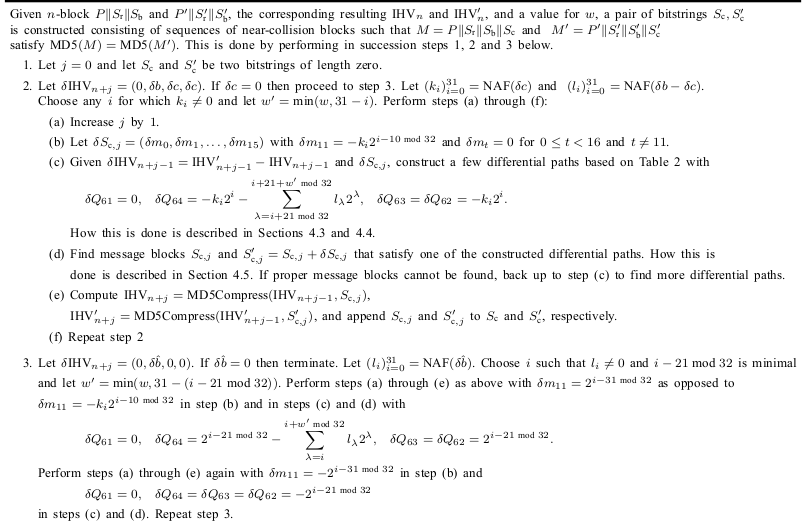
\includegraphics[scale=.61]{ncb.png}
  \caption{Algoritme de recherche des blocs de quasi-collisons}
\end{figure}

\begin{figure}[h!]
  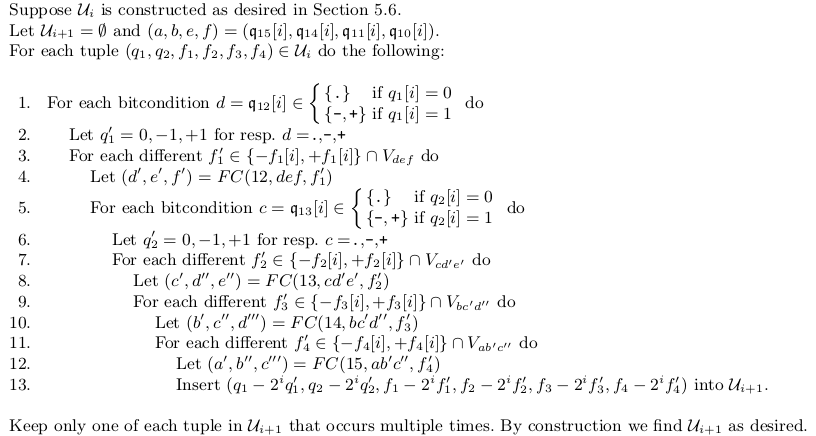
\includegraphics[scale=.61]{ui.png}
  \caption{Algorithme de construction du chemin différentiel}
\end{figure}




\end{document}